\chapter{Building Scanners with \textsl{Ply} \label{chapter:ply-lex}}
\begin{figure}[h] 
\centering
  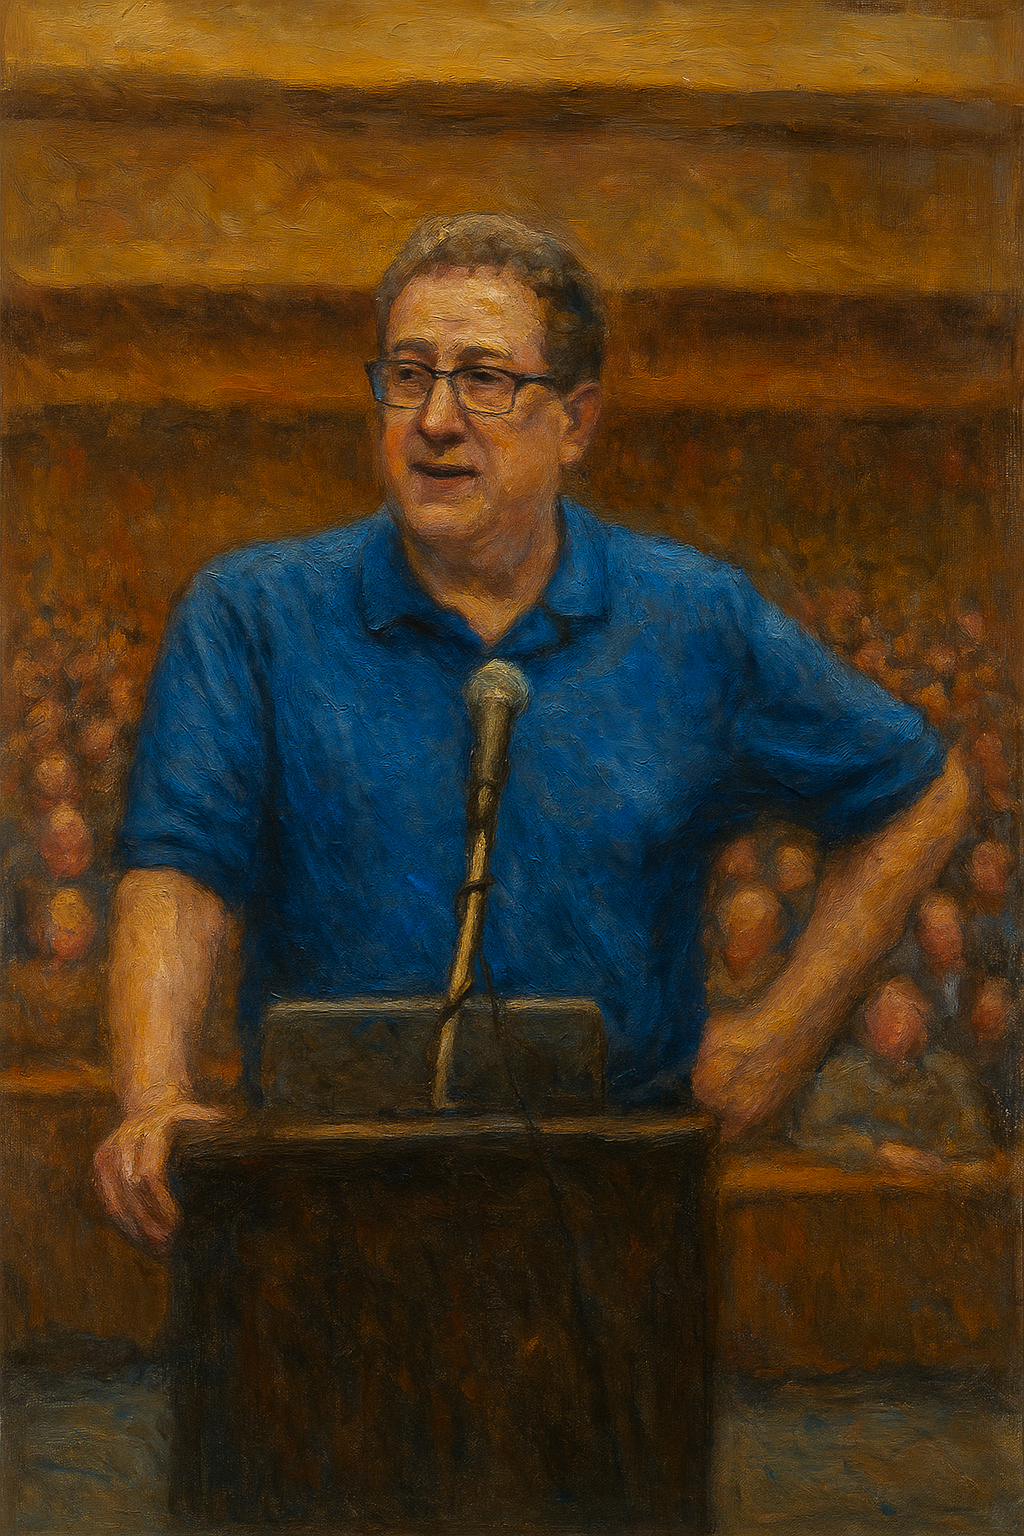
\includegraphics[width=8.5cm]{Abbildungen/david-beazley}
\caption{The creator of Ply, David M.~Beazley.}
\label{fig:david-beazley.png}
\end{figure}


After introducing the concept of regular expressions, we will now explore their practical applications. We
examine the parser generator \texttt{Ply}\index{$\texttt{Ply}$}, which is capable of generating both \textsl{Python}
\emph{scanners} and \textsl{Python} \emph{parsers}.  In this chapter, we will only discuss the generation of
scanners via \texttt{Ply}.
A \textcolor{blue}{scanner}\index{scanner} is a program
designed to segment a given string into a sequence of \emph{tokens}, where a
\textcolor{blue}{token}\index{token} is a contiguous string of characters that logically group together. To
illustrate, consider the input for a \texttt{C}-compiler, which is an \textsc{Ascii}-string representing a
valid \texttt{C} program. The compiler initially organizes these characters into various tokens, including: 

\begin{enumerate}
\item \textcolor{blue}{Keywords} or reserved words, such as, for example, ``\texttt{if}'', ``\texttt{while}'', ``\texttt{for}'', and ``\texttt{switch}''.
\item \textcolor{blue}{Operator symbols}, for example ``\texttt{+}'', ``\texttt{+=}'', ``\texttt{<}'', and ``\texttt{<=}''.
\item \textcolor{blue}{Parentheses}, which include ``\texttt{(}'', ``\texttt{[}'', ``\texttt{\{}'', and their corresponding closing symbols.
\item \textcolor{blue}{Constants}, with \texttt{C} recognizing three types:
    \begin{enumerate}
    \item Numerical constants, such as the integer ``\texttt{42}'' or the floating-point number ``\texttt{1.23e2}''.
    \item String constants enclosed in double quotes, like ``\texttt{\symbol{34}hello\symbol{34}}''.

          Note that the double quote character ``\texttt{\symbol{34}}'' is part of the string constant.
    \item Single-character constants wrapped in single quotes, as in ``\texttt{\symbol{39}a\symbol{39}}''.

          Note that the single quote character ``\texttt{\symbol{39}}'' is part of the character constant.
    \end{enumerate}
\item \textcolor{blue}{Identifiers}, which may serve as variable names, function names, or type names.
\item \textcolor{blue}{Comments}, available in two forms: \textcolor{blue}{Single-line comments} start with
      ``\texttt{//}'' and extend to the end of the line, while \textcolor{blue}{multi-line comments} begin with
      ``\texttt{/*}'' and end with ``\texttt{*/}''. 
\item \textcolor{blue}{Whitespace characters}, such as the \textcolor{blue}{blank character} \texttt{' '}, the \textcolor{blue}{tab} \texttt{'\symbol{92}t'}, the \textcolor{blue}{newline} \texttt{'\symbol{92}n'}, and the \textcolor{blue}{carriage return} \texttt{'\symbol{92}r'}. 

Both whitespace characters and comments are generally discarded by the scanner.
\end{enumerate}

\begin{figure}[!ht]
\centering
\begin{Verbatim}[ frame         = lines, 
                  framesep      = 0.3cm, 
                  firstnumber   = 1,
                  labelposition = bottomline,
                  numbers       = left,
                  numbersep     = -0.2cm,
                  xleftmargin   = 0.8cm,
                  xrightmargin  = 0.8cm,
                ]
    /* Hello World program */
    #include <stdio.h>
    
    int main() {
        printf("Hello World!");
        return 1;
    }
\end{Verbatim}
\vspace*{-0.3cm}
\caption{A straightforward \texttt{C} program.}
\label{fig:hello-world.c}
\end{figure}

\noindent
For a more tangible example, consider Figure \ref{fig:hello-world.c} on page \pageref{fig:hello-world.c}, which
presents a \texttt{C} program that outputs the string ``\texttt{Hello World!}'' along with a newline
character. The scanner processes this program into the subsequent list of tokens:
\pagebreak

\noindent
\hspace*{1.3cm}
   [ ``\texttt{\#}'', ``\texttt{include}'', ``\texttt{<}'', ``\texttt{stdio.h}'', ``\texttt{>}'',
   ``\texttt{int}'', ``\texttt{main}'', ``\texttt{(}'', ``\texttt{)}'', ``\texttt{\{}'',
\\
\hspace*{1.4cm} 
     ``\texttt{printf}'', ``\texttt{(}'', ``\texttt{"Hello World!"}'', ``\texttt{)}'', ``\texttt{;}'', ``\texttt{return}'', ``\texttt{1}'', ``\texttt{;}'', ``\texttt{\}}''
   ]
   \\[0.2cm]
Note that the scanner omits all white space characters, except those that occur inside string constants, as
they are only used to demarcate tokens.  Furthermore, the comment has been removed by the scanner.

While it is feasible to manually create a scanner, using a \textcolor{blue}{scanner generator} makes the task
considerably simpler. We will explore one such utility in the following section. 

\section{The Structure of a \texttt{Ply} Scanner Specification}
In this section, we explore \href{https://www.dabeaz.com/ply/}{Python Lex-Yacc}, \index{ply} commonly known as
\texttt{Ply}. \index{\texttt{Ply}} According to its \href{https://www.dabeaz.com/ply/}{official webpage},
\\[0.2cm]
\hspace*{1.3cm}
``\texttt{Ply} serves as a lex and yacc parsing toolkit for \textsl{Python}.''
\\[0.2cm]
\href{https://en.wikipedia.org/wiki/Lex_(software)}{Lex} is a popular scanner generator for the programming
language \texttt{C}, while \href{https://en.wikipedia.org/wiki/Yacc}{Yacc} is a parser generator for
\texttt{C}.  The toolkit \texttt{Ply} was developed by
\href{https://www.dabeaz.com/}{David Beazley}. In this section, we focus solely on its capabilities as a
scanner generator. In Chapter \ref{chapter:ply} we will discuss how to use \texttt{Ply} as a parser generator. 

To illustrate the core components of a \texttt{Ply} scanner specification, we consider a simple example that
tokenizes arithmetic expressions. This example is adapted from the official \texttt{Ply}
\href{https://ply.readthedocs.io/en/latest/ply.html#specification-of-tokens}{documentation}. A \texttt{Ply}
scanner specification generally consists of three key parts, as demonstrated in Figure
\ref{fig:Ply-Example.ipynb}: 
\begin{enumerate}
\item The module \texttt{ply.lex} contains the definition of the function \texttt{ply.lex.lex()}
      that is able to generate a scanner.
      Therefore, this module is imported in line 1.
\item The first part of a scanner specification is the \blue{token declaration section}.
      Syntactically, this is just a list containing the names of all tokens.  Note that all token names have to
      start with a capital 
      letter.

      In Figure \ref{fig:Ply-Example.ipynb} the token declaration section extends from line 3 to line 11.
\item The second part contains the \blue{token definitions}.  There are two kinds of token definitions:
      \begin{enumerate}
      \item \blue{Immediate token definitions} \index{immediate token definition} have the following form:
            \\[0.2cm]
            \hspace*{1.3cm}
            \texttt{t\_\textsl{NAME} = r'\textsl{regexp}'}
            \\[0.2cm]
            Here \textsl{NAME} has to be one of the names declared in the declaration section and
            \textsl{regexp} is a regular expression using the syntax that is specified in the 
            \textsl{Python} \href{https://docs.python.org/3/library/re.html}{\texttt{re}} module.
      \item \blue{Functional token definitions} \index{functional token definitions} are syntactically
            \textsl{Python function definitions} and have the following form:
            \\[0.2cm]
            \hspace*{1.3cm}
            \texttt{def t\_\textsl{NAME}(t):} \\
            \hspace*{2.05cm}
            \texttt{r'\textsl{regexp}'} \\
            \hspace*{2.8cm} $\vdots$ \\[0.2cm]
            Here, the vertical dots \ ``$\;\vdots\;$'' \ denote any \textsl{Python} code, while
            \textsl{NAME} has to be one of the token names declared in the declaration section and
            \textsl{regexp} is a regular expression.
            
            The functional token definition shown in line 20--23 takes a token \texttt{t} as its
            argument.  This token has the attribute \texttt{t.value}, which refers to the string that has been
            recognized as this token.  In this case, this string is a sequence of digits that can be
            interpreted as a number.  In line 22 the function  \texttt{t\_NUMBER} converts this string into a
            number and stores this number as the attribute \texttt{t.value}.  Finally, the token \texttt{t}
            itself is returned.  This is a typical case where we need a functional token definition since we 
            want to modify the token that is returned.
      \end{enumerate}
      In Figure \ref{fig:Ply-Example.ipynb} the token definitions start in line 13 and end in line 23.
\item The third part deals with the handling of newlines, ignored characters, and scanner errors.
  \begin{enumerate}
  \item A \texttt{Ply} input file may contain the definition of the function \texttt{t\_newline}.
        This function is supposed to deal with newlines contained in the input.  The main purpose of this
        function is to set the  
        counter \texttt{t.lexer.lineno}.  Every token \texttt{t} has the attribute \texttt{t.lexer}, which is a
        reference to the scanner object.  In turn, the scanner object has the attribute \texttt{lineno}, which
        is supposed to be an integer containing the number of the line currently scanned.  This integer starts
        at the value $1$.  Every time a newline is read it should be incremented.

        In line 26 the regular expression \texttt{r'\symbol{92}n+'} matches any positive number of newlines.
        Hence the counter \texttt{lineno} has to be incremented by the length of the string \texttt{t.value.}

        Note that the function \texttt{t\_newline} does \underline{not} return a token.
  \item Line 29 specifies that both blanks and tabs should be ignored by the scanner.
        Note that the string 
        \\[0.2cm]
        \hspace*{1.3cm}
        ``\texttt{' \symbol{92}t'}'' 
        \\[0.2cm]
        is \underline{not} interpreted as a regular expression
        but rather as a list of its characters.  Furthermore, this is not a raw string and must not be prefixed
        with the character ``\texttt{r}'', for otherwise the character sequence ``\texttt{\symbol{92}t}'' would not be
        interpreted as a tab symbol.
  \item The function \texttt{t\_error} deals with characters that can not be recognized.
        An error message is printed and the call \texttt{t.lexer.skip(1)} discards the character that could not be
        matched. 
  \end{enumerate}
\item In line 35 the function \texttt{lex.lex} creates the scanner that has been specified.
\item Line 38 shows how data can be fed into this scanner.
\item In order to use this scanner we can just iterate over it as shown in line 40.  This iteration scans the
      input string using the generated scanner and produces the tokens that are recognized by the scanner one
      by one.  
\end{enumerate}

\begin{figure}[!ht]
\centering
\begin{Verbatim}[ frame         = lines, 
                  framesep      = 0.3cm, 
                  labelposition = bottomline,
                  numbers       = left,
                  numbersep     = -0.2cm,
                  xleftmargin   = 0.8cm,
                  xrightmargin  = 0.8cm,
                ]
    import ply.lex as lex
    
    tokens = [
       'NUMBER',
       'PLUS',
       'MINUS',
       'TIMES',
       'DIVIDE',
       'LPAREN',
       'RPAREN'
    ]
    
    t_PLUS    = r'\+'
    t_MINUS   = r'-'
    t_TIMES   = r'\*'
    t_DIVIDE  = r'/'
    t_LPAREN  = r'\('
    t_RPAREN  = r'\)'
    
    def t_NUMBER(t):
        r'0|[1-9][0-9]*'
        t.value = int(t.value)
        return t
    
    def t_newline(t):
        r'\n+'
        t.lexer.lineno += len(t.value)
    
    t_ignore  = ' \t'
    
    def t_error(t):
        print("Illegal character '%s'" % t.value[0])
        t.lexer.skip(1)
    
    lexer = lex.lex()
    
    data = '3 + 4 * 10 + 007 + (-20) * 2'
    lexer.input(data)
    
    for tok in lexer:
        print(tok)
\end{Verbatim}
\vspace*{-0.3cm}
\caption{A simple scanner Specification for \texttt{Ply}.}
\label{fig:Ply-Example.ipynb}
\end{figure}

\noindent
Executing the program depicted in Figure \ref{fig:Ply-Example.ipynb} yields the following output:

\begin{verbatim}
    LexToken(NUMBER,3,1,0)
    LexToken(PLUS,'+',1,2)
    LexToken(NUMBER,4,1,4)
    % ... (rest of the output)
    LexToken(NUMBER,2,1,27)
\end{verbatim}
The scanner returns tokens as instances of the \texttt{LexToken} class, which possess four distinct attributes:
\begin{enumerate}
\item The \blue{\texttt{type}} attribute indicates the type of the token. It holds a string value that
      corresponds to one of the declared tokens. 
\item The \blue{\texttt{value}} attribute usually contains the recognized string. However, this attribute is
      mutable, allowing for transformations. For instance, the function \texttt{t\_NUMBER} converts this string
      into an integer. 
\item The \blue{\texttt{lineno}} attribute specifies the line number where the token was identified.
\item The \blue{\texttt{lexpos}} attribute serves as a counter, incremented for each character read.
\end{enumerate}

\homeworkEng
Install \texttt{Ply} and verify that the previously presented example operates as expected.
The program \texttt{Ply} can be installed via the following command provided the appropriate \texttt{conda}
environment has already been activated:
\\[0.2cm]
\hspace*{1.3cm}
\texttt{conda install -c conda-forge ply}

\section{The Syntax of Regular Expressions in \textsl{Python}}
In the preceding chapter, we introduced regular expressions using a minimalistic syntax. While this simplicity
is advantageous for the theoretical discussions in the upcoming chapter---where we explore the implementation of
regular expressions via finite state machines---it can be limiting in practical applications. To address this,
the \textsl{Python} module \blue{\textsl{re}} offers various syntactic abbreviations that facilitate the
use of complex regular expressions in a more concise manner. For an in-depth look at these features, I
have authored a brief tutorial at 
\\[0.2cm]
\hspace*{-1.3cm}
\href{https://github.com/karlstroetmann/Formal-Languages/blob/master/Python/Chapter-03/02-Regexp-Tutorial.ipynb}{https://github.com/karlstroetmann/Formal-Languages/blob/master/Python/Chapter-3/02-Regexp-Tutorial.ipynb}
\\[0.2cm]
that focuses on the key aspects of the \texttt{re} module's regular expressions. For an interactive experience,
it is advisable to consult this tutorial directly. 

The web page \href{https://regex101.com}{regex101.com} can be used to test regular expressions for
various programming languages.  Furthermore the web page
\href{https://regexlearn.com/de/learn/regex101}{https://regexlearn.com/de/learn/regex101} provides a free
interactive tutorial for regular expressions.

\section{A Complex Example: Evaluating an Exam}
This sections presents a more complex example that shows some of the power of \texttt{Ply}.  The
task at hand is the evaluation of an exam.  When I mark an exam I create a file that has a format
similar to the example shown in Figure \ref{fig:result.txt}. 

\begin{figure}[!h]
\centering
\begin{Verbatim}[ frame         = lines, 
                  framesep      = 0.3cm, 
                  labelposition = bottomline,
                  numbers       = left,
                  numbersep     = -0.2cm,
                  xleftmargin   = 0.8cm,
                  xrightmargin  = 0.8cm,
                  commandchars  = \\\{\}
                ]
    Class: Algorithms and Complexity
    Group: TINF22AI1
    MaxPoints = 60
   
    Exercise:      1. 2. 3. 4. 5. 6.
    Jim Smith:     9 12 10  6  6  0
    John Slow:     4  4  2  0  -  -
    Susi Sorglos:  9 12 12  9  9  6
\end{Verbatim}
\vspace*{-0.3cm}
\caption{Results of an Exam}
\label{fig:result.txt}
\end{figure}

\begin{enumerate}
\item The first line contains the keyword ``\texttt{Class}'', a colon ``\texttt{:}'', and then the
      name of the lecture. 
\item The second line specifies the group that has taken the exam.
\item The third line specifies the number of points that are necessary to obtain the best mark.
\item The fourth line is empty.
\item The fifth line numbers the exercises.
\item After that, there is a table.  Every row in this table lists the scores achieved by a student
      for each of the exercises.  The name of each student is at the beginning of each row.  The
      name is followed by a colon and after that there is a list of the scores achieved for each
      exercise.  If an exercise has not been attempted at all, the corresponding column contains a hyphen
      ``\texttt{-}''.
\end{enumerate}
I have written a \textsl{Jupyter notebook} that is able to evaluate data of this kind.
You can find the notebook here:
\\[0.2cm]
\hspace*{-1.3cm}
\href{https://github.com/karlstroetmann/Formal-Languages/blob/master/Python/Chapter-03/03-Exam-Evaluation.ipynb}{https://github.com/karlstroetmann/Formal-Languages/blob/master/Python/Chapter-03/03-Exam-Evaluation.ipynb}

\section{Scanner States}
Sometimes, regular expressions are not quite enough and it is beneficial for the scanner to have different
states.  The following example illustrates this.  We will develop a program that is able to convert an 
\textsc{Html} file into a pure text file.  This program is actually quite useful: Some years ago I
had a student who was blind.  If he read a web page, he would use his Braille display.  For him,
the \textsc{Html} markup was of no use so if the markup was removed, he could read web pages faster.
In order to develop the program to remove \textsc{Html} tags, we have to use \blue{scanner states}.
\index{scanner states}  The idea behind scanner states is that the scanner can use different regular
expressions for different parts of the input.  For example, the header of an \textsc{Html} file, i.e.~the part
that is between the \texttt{<head>} and \texttt{</head>} tags, can just be
skipped.  On the other hand, the text inside the \texttt{<body>} and \texttt{</body>} tags needs to be echoed
after any remaining tags have been removed.  The easiest way to achieve this is by using scanner states and
switching between them.  The following notebook shows how this can be done:
\\[0.2cm]
\hspace*{-1.3cm}
\href{https://github.com/karlstroetmann/Formal-Languages/blob/master/Python/Chapter-03/04-Html2Text.ipynb}{https://github.com/karlstroetmann/Formal-Languages/blob/master/Python/Chapter-03/04-Html2Text.ipynb}
\\

\exerciseEng
The purpose of the following exercise is to transform \href{http://www.latex-project.org}{\LaTeX} into 
\href{https://www.tutorialspoint.com/mathml/index.htm}{\textsc{MathML}}.  \LaTeX\ is a document markup language
that is especially well suited to present text that contains mathematical formulas.  In fact, these
lecture notes have all been typeset using \LaTeX.  \textsc{MathML} is the part of \textsc{Html} that
deals with the representation of mathematical formulas.  As \LaTeX\ provides a very rich
document markup language and we can only afford to spend a few hours on this exercise, we confine
ourselves to a small subset of \LaTeX.  Figure \ref{fig:input.tex} on page \pageref{fig:input.tex}
shows the example input file that we want to transform in \textsc{Html}.  If this example file is
typeset using \LaTeX, it is displayed as shown in Figure \ref{fig:input.pdf} on page
\pageref{fig:input.pdf}.  The program that you are
going to develop should transform the \LaTeX\ input file into an \textsc{Html} file.  For your
convenience, all these files are available in the github directory 
\\[0.2cm]
\hspace*{1.3cm}
\href{https://github.com/karlstroetmann/Formal-Languages/tree/master/Python/Chapter-03/05-LaTeX2HTML}{\texttt{Python/LaTeX2HTML}}.
\\[0.2cm]
This directory contains also the \textsl{Jupyter} notebook 
\href{https://github.com/karlstroetmann/Formal-Languages/blob/master/Python/Chapter-03/05-LaTeX2HTML/LaTeX2HTML.ipynb}{\texttt{LaTeX2HTML.ipynb}}.
This notebook contains lots of predefined functions that are useful in order to solve the given task.

\begin{figure}[!ht]
  \centering
\begin{verbatim}
    \documentclass{article}
    \begin{document}
    The sum of the squares of the first $n$ natural numbers is given as:
    $$ \sum\limits_{i=1}^{n} i^{2} = \frac{1}{6} \cdot n \cdot (n+1) \cdot (2\cdot n + 1). $$
    According to Pythagoras, the length of the hypotenuse of a right triangle is
    the square root of the squares of the length of the two catheti:
    $$ c = \sqrt{a^{2} + b^{2}}.  $$
    The area of a circle is given as 
    $$  A = \pi \cdot r^{2},   $$ 
    while its circumference satisfies
    $$ C = 2 \cdot \pi \cdot r.  $$
    \end{document}
    \end{verbatim}
  \caption{An example \LaTeX\ input file.}
  \label{fig:input.tex}
\end{figure}

\begin{figure}[!ht]
  \centering
  \framebox{
  \begin{minipage}{0.8\linewidth}
    The sum of the squares of the first $n$ natural numbers is given as:
    $$ \sum_{i=1}^{n} i^{2} = \frac{1}{6} \cdot n \cdot (n+1) \cdot (2\cdot n + 1). $$
    According to Pythagoras, the length of the hypotenuse of a right triangle is
    the square root of the squares of the length of the two catheti:
    $$ c = \sqrt{a^{2} + b^{2}}.  $$
    The area $A$ of a circle is given as 
    $$  A = \pi \cdot r^{2},   $$ 
    while its circumference satisfies
    $$ C = 2 \cdot \pi \cdot r.  $$   
  \end{minipage}}
  \caption{Output produced by the \LaTeX\ file shown in Figure \ref{fig:input.tex}}
  \label{fig:input.pdf}
\end{figure}

In order to do this exercise, you have to understand a little bit about \LaTeX\ and about 
\textsc{MathML}.  In the following, we discuss those features of these two language that are needed in order to
solve the given problem.
\begin{enumerate}
\item A \LaTeX\ input file has the following structure:
      \begin{enumerate}
      \item The first line list the type of the document.  In our example, it reads
            \\[0.2cm]
            \hspace*{1.3cm}
            \texttt{\symbol{92}documentclass\{article\}}.
            \\[0.2cm]
            This line will be transformed into the following \textsc{Html}:
            \begin{verbatim}
 <html>
 <head>
 <script type="text/javascript"
 src="http://cdn.mathjax.org/mathjax/latest/MathJax.js?config=TeX-AMS-MML_HTMLorMML">
 </script>
 </head>
            \end{verbatim}
            Here, the \texttt{<script>} tag is necessary in order for the \textsc{MathML} 
            to be displayed correctly.
      \item The next line has the form:
            \\[0.2cm]
            \hspace*{1.3cm}
            \texttt{\symbol{92}begin\{document\}}
            \\[0.2cm]
            This line precedes the content and should be translated into the tag
            \\[0.2cm]
            \hspace*{1.3cm}
            \texttt{<body>}.
      \item After that, the \LaTeX\ file consists of text that contains mathematical formula.
      \item The \LaTeX\ input file finishes with a line of the form
            \\[0.2cm]
            \hspace*{1.3cm}
            \texttt{\symbol{92}end\{document\}}.
            \\[0.2cm]
            This line should be translated into the tags
            \\[0.2cm]
            \hspace*{1.3cm}
            \texttt{</body></html>}.
      \end{enumerate}
\item In \LaTeX, an inline formula is started and ended with a single dollar symbol
      ``\texttt{\symbol{36}}''.  
      In \textsc{MathML}, an inline formula is written as
      \\[0.2cm]
      \hspace*{1.3cm}
      \texttt{<math xmlns="http://www.w3.org/1998/Math/MathML" display='inline'>$\cdots$</math>}.
      \\[0.2cm]
      Here, I have used ``$\cdots$'' to represent the mathematical content of the formula.
\item In \LaTeX, a formula that is displayed in its own line is started and ended with the string
      ``\texttt{\symbol{36}\symbol{36}}''.  
      In \textsc{MathML}, these formulas\ are called \blue{block formulas} and are written as
      \\[0.2cm]
      \hspace*{1.3cm}
      \texttt{<math xmlns="http://www.w3.org/1998/Math/MathML" display='block'>$\cdots$</math>}.
      \\[0.2cm]
      Again, I have used ``$\cdots$'' to represent the mathematical content of the formula.
\item While in \LaTeX\ a mathematical variable does not need any special markup, in \textsc{MathMl}
      a mathematical variable is written using the tags 
      \texttt{<mi>} and \texttt{</mi>}.  For example, the mathematical variable $n$ is written as    
      \\[0.2cm]
      \hspace*{1.3cm}
      \texttt{<mi>n</mi>}.
\item While in \LaTeX\ a number does not need any special markup, in \textsc{MathMl}
      a number is written using the tags 
      \texttt{<mn>} and \texttt{</mn>}.  For example, the number $3.14159$ is written as    
      \\[0.2cm]
      \hspace*{1.3cm}
      \texttt{<mn>3.14159</mn>}.
\item In \LaTeX\ the mathematical constant $\pi$ is written using the command ``\texttt{\symbol{92}pi}''.
      In \textsc{MathMl}, we have to make use of the \textsc{Html} entity ``\texttt{\&pi;}'' and
      hence we would write $\pi$ as
      \\[0.2cm]
      \hspace*{1.3cm}
      \texttt{<mn>\&pi;</mn>}.
\item In \LaTeX\ the multiplication operator ``$\cdot$'' is written using the command ``\texttt{\symbol{92}cdot}''.
      In \textsc{MathMl}, we have to make use of the \textsc{Html} entity ``\texttt{\&sdot;}'' and
      hence we would write ``$\cdot$'' as
      \\[0.2cm]
      \hspace*{1.3cm}
      \texttt{<mop>\&sdot;</mop>}.
\item While in \LaTeX\ most operator symbols stand for themselves, in \textsc{MathMl}
      an operator is surrounded by the tags 
      \texttt{<mop>} and \texttt{</mop>}.  For example, the operator $+$ is written as    
      \\[0.2cm]
      \hspace*{1.3cm}
      \texttt{<mop>+</mop>}.
\item In \LaTeX, raising an expression $e$ to the $n$th power is done using the operator
      ``\texttt{\symbol{94}}''.  Furthermore, the exponent should be enclosed in the curly braces
      ``\texttt{\{}'' and ``\texttt{\}}''.  For example, the code to produce the term $x^2$ is
      \\[0.2cm]
      \hspace*{1.3cm}
      \texttt{x\symbol{94}\{2\}}.
      \\[0.2cm]
      In \textsc{MathMl}, raising an expression to a power is achieved using the tags
      \texttt{<msup>} and \texttt{</msup>}.  For example, in order to display the term $x^2$, we
      have to write  
      \\[0.2cm]
      \hspace*{1.3cm}
      \texttt{<msup><mi>x</mi><mn>2</mn></msup>}.
\item In \LaTeX, taking the square root of an expression is done using the command
      ``\texttt{\symbol{92}sqrt}''.  The argument has to be enclosed in curly braces.
      For example, in order to produce the output $\sqrt{a+b}$, we have to write
      \\[0.2cm]
      \hspace*{1.3cm}
      \texttt{\symbol{92}sqrt\{a+b\}}.
      \\[0.2cm]
      In \textsc{MathMl}, taking the square root makes use of the tags \texttt{<msqrt>} 
      and \texttt{</msqrt>}.  The example shown above can be written as
      \\[0.2cm]
      \hspace*{1.3cm}
      \texttt{<msqrt><mi>a</mi><mop>+</mop><mi>b</mi></msqrt>}.
\item In \LaTeX, writing a fraction is done using the command
      ``\texttt{\symbol{92}frac}''.  This command takes two arguments, the numerator and the
      denominator.  Both of these have to be enclosed in curly braces.
      For example, in order to produce the output $\frac{a+b}{2}$, we have to write
      \\[0.2cm]
      \hspace*{1.3cm}
      \texttt{\symbol{92}frac\{a+b\}\{2\}}.
      \\[0.2cm]
      In \textsc{MathMl}, a fraction is created via the tags \texttt{<mfrac>} 
      and \texttt{</mfrac>}.  Additionally, if the arguments contain more than a single element,
      each of them has to be enclosed in the tags \texttt{<mrow>} and \texttt{</mrow>}.
      The example shown above can be written as
      \\[0.2cm]
      \hspace*{1.3cm}
      \texttt{<mfrac><mrow><mi>a</mi><mop>+</mop><mi>b</mi></mrow><mn>2</mn></mfrac>}.
\item In \LaTeX, writing a sum is done using the command
      ``\texttt{\symbol{92}sum\symbol{92}limits}''.  
      This command takes two arguments:  The first argument gives the indexing variable together
      with its lower bound, while the second argument gives the upper bound.  The first argument
      is started using the string ``\texttt{\_\{}'' and ended using the string ``\texttt{\}}'',
      while the second argument is started using the string ``\texttt{\symbol{94}\{}'' and ended using the
      string ``\texttt{\}}''.  For example, in order to produce the output 
      \\[0.2cm]
      \hspace*{1.3cm}
      $\displaystyle\sum\limits_{i=1}^{n} i$,
      \\[0.2cm]
      we have to write
      \\[0.2cm]
      \hspace*{1.3cm}
      \texttt{\symbol{92}sum\symbol{92}limits\_\{i=1\}\symbol{94}\{n\} i}.
      \\[0.2cm]
      In \textsc{MathMl}, a sum with lower and upper limits is created via the tags
      \texttt{<munderover>} and \texttt{</munderover>} and the \textsc{Html} entity ``\texttt{\&sum}''.
      The tag \texttt{munderover} takes three arguments:
      \begin{enumerate}
      \item The first argument is the operator, so in this case it is the entity ``\texttt{\&sum}''.
      \item The second argument initializes the indexing variable of the sum.
      \item The third argument provides the upper bound.
      \end{enumerate}
      The second argument usually contains more than a single item and therefore has to be enclosed 
      in the tags \texttt{<mrow>} and \texttt{</mrow>}.
      Hence, the example shown above would be written as follows:
      
    \begin{verbatim}
    <munderover>
        <mo>&sum;</mo>
        <mrow>
            <mi>i</mi> <mo>=</mo> <mn>1</mn>
        </mrow>
        <mi>n</mi>
    </munderover>
    \end{verbatim}
\end{enumerate}

\remarkEng
The most important problem that you have to solve is the following:  Once you encounter a closing brace
``\texttt{\}}'' you have to know whether this brace closes the argument of a square root, a
fraction, a sum, or an exponent.  You should be aware that, for example, square roots and fractions
can be nested.  Hence, it is not enough to have a single variable that remembers whether you are
parsing, say, a square root or a fraction.  Instead, every time you encounter a string like, e.g.
\\[0.2cm]
\hspace*{1.3cm}
\texttt{\symbol{92}sqrt\{} \quad or \quad \texttt{\symbol{92}frac\{},
\\[0.2cm]
you should store the current state on a stack and set the new state according to whether you have just seen the
keyword ``\texttt{\symbol{92}frac}'' or ``\texttt{\symbol{92}sqrt}'' or whatever caused the
curly brace to be opened.  When you encounter a closing brace ``\texttt{\}}'', you should 
restore the state to its previous value by looking up this value from the stack.  
\eox

\section{Check your Understanding}
\begin{enumerate}[(a)]
\item How are regular expressions defined in \textsl{Python}?
\item Do you understand the structure of a \texttt{Ply} scanner specification?
\item Are you able to use \texttt{Ply} to write a program that reads a given text, finds all numbers inside
      this text that are followed by a $\texttt{\$}$ symbol and that then converts these numbers to their equivalent
      value in \texttt{\euro{}}?  Assume that $1 \mathtt{\$} = 0.85 \texttt{\euro{}}$.
\end{enumerate}



%%% Local Variables: 
%%% mode: latex
%%% TeX-master: "formal-languages.tex"
%%% End: 
